\documentclass[a4paper,11pt]{article}

%%%%%%%%%%%%%%%%%%%%%%%%%%%%%%%%%%%%%%%%%%%%%%%%%%%%%%%%%%%%%%%%%%%%%%%%
% Paquetes utilizados
%%%%%%%%%%%%%%%%%%%%%%%%%%%%%%%%%%%%%%%%%%%%%%%%%%%%%%%%%%%%%%%%%%%%%%%%

% Gráficos complejos
\usepackage{graphicx}
\usepackage{caption}
\usepackage{subcaption}
\usepackage{placeins}

% Soporte para el lenguaje español
\usepackage{textcomp}
\usepackage[utf8]{inputenc}
\usepackage[T1]{fontenc}
\DeclareUnicodeCharacter{B0}{\textdegree}
\usepackage[spanish]{babel}

% Código fuente embebido
\usepackage{listings}
\lstset{
  basicstyle=\footnotesize,
  showspaces=false,
  showstringspaces=false,
  breaklines=true,
  frame=single
}

% Matemáticos
\usepackage{amssymb,amsmath}

% Tablas complejas
\usepackage{multirow}

% Formato de párrafo
\setlength{\parskip}{1ex plus 0.5ex minus 0.2ex}

% Formato de encabezados y pies de página
\usepackage{fancyhdr}
\fancyhead{}
\fancyfoot{}
\setlength\headheight{40pt}
\fancyhead[L]{
  Facultad de Ingeniería \\ 
  Universidad de Buenos Aires
}
\fancyhead[R]{
  71.14 - Modelos y Optimización I \\
  Trabajo Práctico - 2° entrega
}
\fancyfoot[C]{
  \thepage
}
\pagestyle{fancy}

%%%%%%%%%%%%%%%%%%%%%%%%%%%%%%%%%%%%%%%%%%%%%%%%%%%%%%%%%%%%%%%%%%%%%%%%
% Documento
%%%%%%%%%%%%%%%%%%%%%%%%%%%%%%%%%%%%%%%%%%%%%%%%%%%%%%%%%%%%%%%%%%%%%%%%
\title{\textbf{Trabajo Práctico} - 2° entrega}
\author{Andrés Gastón Arana, \textit{P. 86.203}}
\date{}

\begin{document}

\maketitle
\clearpage

\part{Modelo propuesto por el grupo de trabajos prácticos}

\section{Resolución por LINGO}

Para la resolución del modelo planteado en la primer entrega del trabajo
práctico se utilizó \textit{LINGO}, una suite de software de resolución de
modelos de programación lineal desarrollada por la misma empresa que implementó
\textit{LINDO}. La sintáxis de los archivos de modelos, así como la salida del
programa al resolver el modelo, son completamente compatibles y equivalentes a
las utilizadas por \textit{LINDO}, denominado \textit{LINDO Classic} por la
empresa.

A continuación se presenta el modelo en la sintaxis propia de la herramienta
elegida:

\lstinputlisting{lingo/general.lng}

Cuando se ejecutó el software de resolución de modelos lineales en el modelo,
se obtuvo el siguiente resultado:

\lstinputlisting{lingo/general.out}

\section{Análisis de los resultados}

El modelo arrojo los siguientes resultados:

\begin{itemize}

\item Se producen \(5000kg\) de producto P y \(8000kg\) de producto C. Se
  decide no producir producto G en lo absoluto.

\item La materia prima utilizada para fabricar los productos son \(12166.67kg\)
  de maiz y \(833.33kg\) de cáscara de arroz. Se decide no utilizar ninguna
  otra materia prima, incluso cuando esto significa que \(5166.66kg\) de maiz
  se están comprando con recargo.

\item Se dedican \(4166.66kg\) y \(833.33kg\) de cáscara de arroz para producir
  producto P. Esto significa que se utiliza lo mínimo indispensable de maiz
  disponible para cumplir con los requerimientos protéicos para el producto.

\item Se dedican \(8000kg\) de maiz para producir producto C. Esto se debe a
  que no se puede utilizar cáscara de arroz en este caso, dado que el maiz
  apenas cubre el requerimiento protéico necesario para este producto.

\end{itemize}

Por otro lado, las restricciones de demanda de producto P, demanda de producto
C y la cantidad de maiz prepactada a valor reducido tienen un valor marginal
positivo. Esto indica que aumentar cualquiera de las cantidades asociadas (las
demandas máximas de producto P o C y la cantidad de maiz disponible a precio
reducido) tendrá un efecto positivo en el funcional maximizado.

Particularmente, el valor marginal para la demanda de producto P es \(7.58\),
el de la demanda de producto C es \(4\), y el correspondiente al pactado de
maiz es \(0.5\). Con estos datos, parecería ser conveniente invertir en algún
tipo de campaña de publicidad para aumentar la demanda de producto P.

\clearpage
\part{Modelo propuesto por el turno}

\section{Resolución gráfica} \label{sec:grafica}

En la figura \ref{fig:resolucion} se puede observar el dominio graficado del
modelo expuesto en la primer entrega.

\begin{figure}[h!]
  \centering
  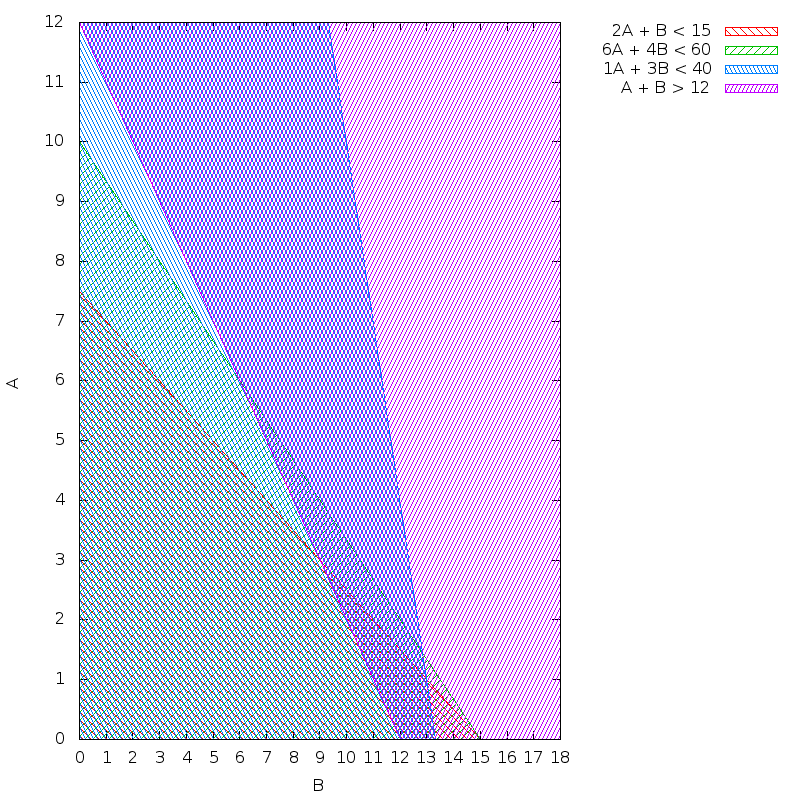
\includegraphics[width=\textwidth]{graphic/output.png}
  \caption{Grafico del dominio del modelo matemático}\label{fig:resolucion}
\end{figure}

\FloatBarrier

Los vértices del poliedro se resumen en el cuadro \ref{tab:resolucion}.

\begin{table}[h!]
\centering
\begin{tabular}{ | c | c | c | }
  \hline
  A & B     & Z (\$) \\ \hline
  0 & 13.33 & 39999.99\\ \hline
  1 & 13    & 44000 \\ \hline
  3 & 9     & 42000 \\ \hline
  0 & 12    & 36000 \\ \hline
\end{tabular}
\caption{Vértices de optimización en la resolución gráfica}\label{tab:resolucion}
\end{table}

\FloatBarrier

Como puede observarse, el máximo funcional Z es en el punto \(A = 1\) y \(B =
13\), con un valor funcional de \(\$44000\).

\section{Resolución por Simplex} \label{sec:simplex}

En el cuadro \ref{tab:simplex} se presentan las tablas intermedias y la
resolución final de la aplicación del método simplex. Las ecuaciones son las
mismas que serán detalladas en la descripción del modelo simplificado de la
sección \ref{sec:lingo}, pero pueden resolverse como siguen:

\[
  2x_1 + x_2 + x_3 = 15
\]

\[
  6x_1 + 4x_2 + x_4 = 60
\]

\[
  x_1 + 3x_2 + x_5 = 40
\]

\[
  x_1 + x_2 - x_6 + m = 12
\]

\[
  \text{MAX z} = 5000x_1 + 3000x_2 - Mm
\]

\begin{table}[h!]
\centering
\begin{tabular}{ | c | c | c || c | c | c | c | c | c | c || c | }
  \hline
  C          & X       & B    & \(A_1\)   & \(A_2\)     & \(A_3\)     & \(A_4\) & \(A_5\) & \(A_6\) & \(A_m\) & \(\theta\) \\ \hline
  0          & \(x_3\) & 15   & 2         & 1           & 1           & 0       & 0       & 0       & 0       & \(7.5\) \\ \hline
  0          & \(x_4\) & 60   & 6         & 4           & 0           & 1       & 0       & 0       & 0       & 10 \\ \hline
  0          & \(x_5\) & 40   & 1         & 3           & 0           & 0       & 1       & 0       & 0       & 40 \\ \hline
 -M          & \(m\)   & 12   & 1         & 1           & 0           & 0       & 0       & -1      & 1       & 12 \\ \hline \hline
             &         &      & -M - 5000 & -M - 3000   & 0           & 0       & 0       & M       & 0       & \\ \hline \hline
  5000       & \(x_1\) & 7,5  & 1         & 0,5         & 0,5         & 0       & 0       & 0       & 0       & 15 \\ \hline
     0       & \(x_4\) & 15   & 0         & 1           & -3          & 1       & 0       & 0       & 0       & 15 \\ \hline
     0       & \(x_5\) & 32,5 & 0         & 2,5         & -0,5        & 0       & 1       & 0       & 0       & 13 \\ \hline
    -M       & \(m\)   & 4,5  & 0         & 0,5         & -0,5        & 0       & 0       & -1      & 1       & 9 \\ \hline \hline
             &         &      & 0         & -500 - 0,5M & 2500 + 0,5M & 0       & 0       & M       & 0       & \\ \hline \hline
    5000     & \(x_1\) & 3    & 1         & 0           & 1           & 0       & 0       & 1       & -1      & \\ \hline
       0     & \(x_4\) & 6    & 0         & 0           & -2          & 1       & 0       & 2       & -2      & \\ \hline
        0    & \(x_5\) & 10   & 0         & 0           & 2           & 0       & 1       & 5       & -5      & \\ \hline
      3000   & \(x_2\) & 9    & 0         & 1           & -1          & 0       & 0       & -2      & 2       & \\ \hline \hline
             &         &      & 0         & 0           & 2           & 0       & 0       & 47      & -47 + M & \\ \hline
\end{tabular}
\caption{Tablas simplex para el problema}\label{tab:simplex}
\end{table}

\FloatBarrier

\section{Resolución por LINGO}\label{sec:lingo}

A continuación se presenta el modelo en la sintaxis propia de la herramienta
elegida:

\lstinputlisting{lingo/turno.lng}

Cuando se ejecutó el software de resolución de modelos lineales en el modelo,
se obtuvo el siguiente resultado:

\lstinputlisting{lingo/turno.out}

\section{Análisis de los resultados}

La resolución del modelo arrojo los siguientes resultados:

\begin{itemize}

  \item Se decide instalar 13 máquinas B y una máquina tipo A, con un funcional
    maximizado en \(\$44000\).

  \item Tanto la memoria RAM como el tiempo de procesador son recursos
    saturados. El valor marginal de la RAM, siendo mayor que el del procesador,
    parece indicar que este es el recurso a conseguir para mejorar el
    funcional.

\end{itemize}

\end{document}
